\documentclass{beamer}
\usepackage{amsmath}
\usepackage[english]{babel} %set language; note: after changing this, you need to delete all auxiliary files to recompile
\usepackage[utf8]{inputenc} %define file encoding; latin1 is the other often used option
\usepackage{csquotes} % provides context sensitive quotation facilities
\usepackage{graphicx} %allows for inserting figures
\usepackage{booktabs} % for table formatting without vertical lines
\usepackage{textcomp} % allow for example using the Euro sign with \texteuro
\usepackage{stackengine}
\usepackage{wasysym}
\usepackage{tikzsymbols}
\usepackage{textcomp}
\usepackage{xcolor}
\usepackage[dvipsnames]{xcolor}
\usepackage{colortbl}
\usepackage{adjustbox}
\usetikzlibrary{decorations.pathreplacing}
\newcommand{\bubblethis}[2]{
        \tikz[remember picture,baseline]{\node[anchor=base,inner sep=0,outer sep=0]%
        (#1) {\underline{#1}};\node[overlay,cloud callout,callout relative pointer={(0.2cm,-0.7cm)},%
        aspect=2.5,fill=yellow!90] at ($(#1.north)+(-0.5cm,1.6cm)$) {#2};}%
    }%
\tikzset{face/.style={shape=circle,minimum size=4ex,shading=radial,outer sep=0pt,
        inner color=white!50!yellow,outer color= yellow!70!orange}}
%% Some commands to make the code easier
\newcommand{\emoticon}[1][]{%
  \node[face,#1] (emoticon) {};
  %% The eyes are fixed.
  \draw[fill=white] (-1ex,0ex) ..controls (-0.5ex,0.2ex)and(0.5ex,0.2ex)..
        (1ex,0.0ex) ..controls ( 1.5ex,1.5ex)and( 0.2ex,1.7ex)..
        (0ex,0.4ex) ..controls (-0.2ex,1.7ex)and(-1.5ex,1.5ex)..
        (-1ex,0ex)--cycle;}
\newcommand{\pupils}{
  %% standard pupils
  \fill[shift={(0.5ex,0.5ex)},rotate=80] 
       (0,0) ellipse (0.3ex and 0.15ex);
  \fill[shift={(-0.5ex,0.5ex)},rotate=100] 
       (0,0) ellipse (0.3ex and 0.15ex);}

\newcommand{\emoticonname}[1]{
  \node[below=1ex of emoticon,font=\footnotesize,
        minimum width=4cm]{#1};}
\usepackage{scalerel}
\usetikzlibrary{positioning}
\usepackage{xcolor,amssymb}
\newcommand\dangersignb[1][2ex]{%
  \scaleto{\stackengine{0.3pt}{\scalebox{1.1}[.9]{%
  \color{red}$\blacktriangle$}}{\tiny\bfseries !}{O}{c}{F}{F}{L}}{#1}%
}
\newcommand\dangersignw[1][2ex]{%
  \scaleto{\stackengine{0.3pt}{\scalebox{1.1}[.9]{%
  \color{red}$\blacktriangle$}}{\color{white}\tiny\bfseries !}{O}{c}{F}{F}{L}}{#1}%
}
\usepackage{fontawesome} % Social Icons
\usepackage{epstopdf} % allow embedding eps-figures
\usepackage{tikz} % allows drawing figures
\usepackage{amsmath,amssymb,amsthm} %advanced math facilities
\usepackage{lmodern} %uses font that support italic and bold at the same time
\usepackage{hyperref}
\usepackage{tikz}
\usepackage{tcolorbox}

\usefonttheme[onlymath]{serif} %set math font to serif ones

\definecolor{beamerblue}{rgb}{0.2,0.2,0.7} %define beamerblue color for later use

%%% defines highlight command to set text blue
\newcommand{\highlight}[1]{{\color{blue}{#1}}}


%%%%%%% commands defining backup slides so that frame numbering is correct

\newcommand{\backupbegin}{
   \newcounter{framenumberappendix}
   \setcounter{framenumberappendix}{\value{framenumber}}
}
\newcommand{\backupend}{
   \addtocounter{framenumberappendix}{-\value{framenumber}}
   \addtocounter{framenumber}{\value{framenumberappendix}}
}

%%%% end of defining backup slides

%Specify figure caption, see also http://tex.stackexchange.com/questions/155738/caption-package-not-working-with-beamer
\setbeamertemplate{caption}{\insertcaption} %redefines caption to remove label "Figure".
%\setbeamerfont{caption}{size=\scriptsize,shape=\itshape,series=\bfseries} %sets figure  caption bold and italic and makes it smaller

\newtcolorbox{boxA}{
    fontupper = \bf,
    boxrule = 1.5pt,
    colframe = black % frame color
}
\newtcolorbox{boxB}{
    boxrule = 1.5pt,
    colframe = blue!70!black,, % frame color
    colback = blue!7!white,
}

\usetheme{Boadilla}

% --------------------
% Overall information
% --------------------
\title[Economía I]{Economía I \vspace{4mm}
\\ Magistral 19: Teoría de crecimiento}
\date{}
\author[Franco Riottini]{Riottini Franco}
\vspace{0.4cm}
\institute[]{Universidad de San Andrés} 


\begin{document}

\begin{frame}
\titlepage
\centering


\includegraphics[scale=0.2]{../Figures/logoUDESA.jpg} 
\end{frame}

\begin{frame}{Crecimiento del GDP}
    \begin{figure} [H]   
        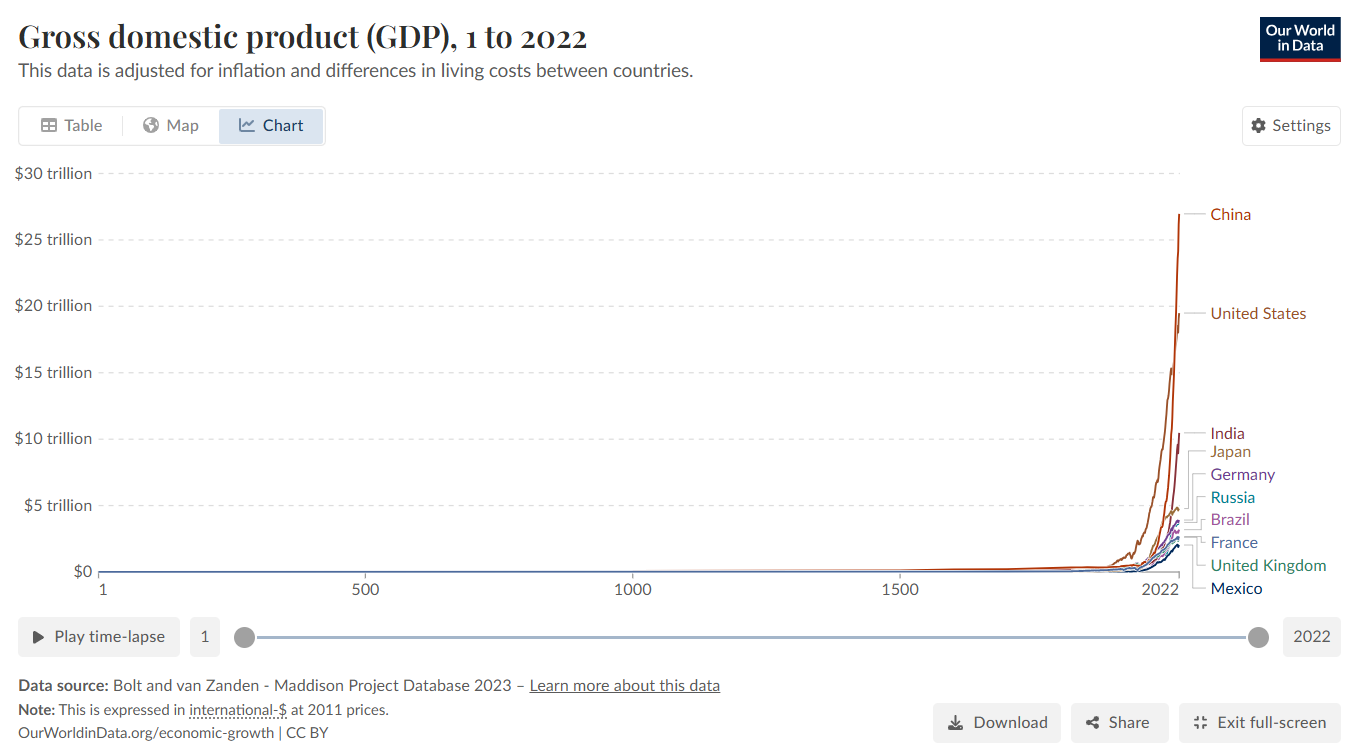
\includegraphics[scale=0.4]{../Figures/gdp_growth_ourworldindata.png}
    \end{figure}
\end{frame}

% \begin{frame}{Crecimiento del GDP per cápita}
%     \begin{figure} [H]   
%         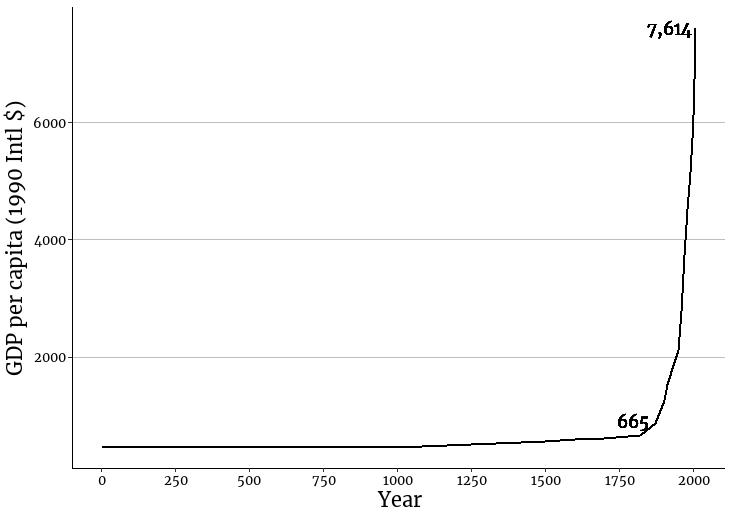
\includegraphics[scale=0.5]{../Figures/C17.1.png}
%     \end{figure}
% \end{frame}

\begin{frame}{La Gran Divergencia}
    \begin{itemize}
        \item Hasta 1800, la mayoría de las regiones tenían niveles similares (y bajos) de ingreso per cápita.
        \item A partir del siglo XIX, algunos países despegan (Reino Unido, Europa, EE.UU.).
        \item La brecha entre países ricos y pobres se amplía enormemente.
        \item Este fenómeno se conoce como “La Gran Divergencia”.
        \item Causas principales: industrialización, instituciones inclusivas, tecnología, comercio.
    \end{itemize}
\end{frame}

\begin{frame}{Crecimiento poblacional vs. per cápita}
    \begin{itemize}
        \item El crecimiento económico total tiene dos componentes:
        \begin{itemize}
            \item Aumento de la población (más trabajadores).
            \item \textbf{Aumento del producto por persona (productividad)}.
        \end{itemize}
        \item La “revolución del crecimiento moderno” es que crece el \textbf{PIB per cápita}.
        \item Se rompe la trampa maltusiana: más personas \textbf{y} más riqueza por persona.
        \item Es clave distinguir crecimiento extensivo (más insumos) de intensivo (mejora en productividad).
    \end{itemize}
\end{frame}

\begin{frame}{Factores del crecimiento}
    \begin{center}
        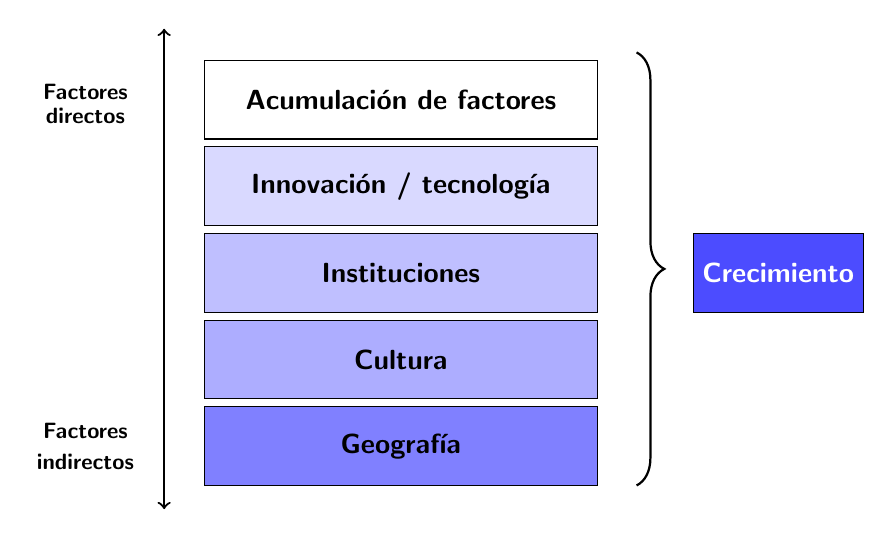
\begin{tikzpicture}[font=\sffamily]

        % Flecha vertical (factores directos e indirectos)
        \draw[thick, <->] (0.5, -0.8) -- (0.5, 5.3);
        \node[] at (-0.5, 4.5) {\footnotesize \textbf{Factores}};
        \node[] at (-0.5, 4.2) {\footnotesize \textbf{directos}};
        \node[] at (-0.5, 0.2) {\footnotesize \textbf{Factores}};
        \node[] at (-0.5, -0.2) {\footnotesize \textbf{indirectos}};

        % Rectángulos de factores
        \node[draw, fill=blue!50, minimum width=5cm, minimum height=1cm, anchor=west] at (1, 0) {\textbf{Geografía}};
        \node[draw, fill=blue!32, minimum width=5cm, minimum height=1cm, anchor=west] at (1, 1.1) {\textbf{Cultura}};
        \node[draw, fill=blue!25, minimum width=5cm, minimum height=1cm, anchor=west] at (1, 2.2) {\textbf{Instituciones}};
        \node[draw, fill=blue!15, minimum width=5cm, minimum height=1cm, anchor=west] at (1, 3.3) {\textbf{Innovación / tecnología}};
        \node[draw, fill=white, minimum width=5cm, minimum height=1cm, anchor=west] at (1, 4.4) {\textbf{Acumulación de factores}};

        % Llave del costado
        \draw[decorate, decoration={brace, amplitude=10pt}, thick] (6.5, 5) -- (6.5, -0.5);

        % Flecha hacia Growth
        \node[draw, fill=blue!70, text=white, minimum width=2cm, minimum height=1cm] at (8.3,2.2) {\textbf{Crecimiento}};


        \end{tikzpicture}
    \end{center}
\end{frame}

\begin{frame}{Momentos clave del despegue}
    \small
    \begin{itemize}
        \item La \textit{Revolución Industrial} ($\sim$1760-1840) cambió la trayectoria del desarrollo.
        \item \textbf{Gran Bretaña lidera}: máquina de vapor, industria textil, ferrocarriles.
        \item Tecnología permitió producción sostenida por encima del crecimiento poblacional.
        \item Comienzan procesos acumulativos: inversión, educación, urbanización, innovación.
        \item Primeros países en industrializarse logran ventajas persistentes (\textit{path dependence}).
        \item Revoluciones institucionales:
        \begin{itemize}
            \scriptsize
            \item \textbf{EE.UU. (1787):} Constitución que limita el poder estatal y protege derechos de propiedad.
            \item \textbf{Francia (1789):} Fin del orden estamental, avance hacia igualdad jurídica y libertad ocupacional.
            \item Cambios políticos crean entornos más predecibles y favorables al emprendimiento.
            \item Los derechos civiles y la división de poderes fortalecen las instituciones inclusivas.
            \item Ejemplos que inspiraron transformaciones institucionales globales.
        \end{itemize}
    \end{itemize}
\end{frame}


\begin{frame}{Cultura y crecimiento}
    \begin{itemize}
        \item La cultura influye en valores como trabajo, ahorro, confianza y cooperación.
        \item \textbf{Max Weber:} la ética protestante y el espíritu del capitalismo.
        \begin{itemize}
            \item El protestantismo (Lutero) es una escisión del catolicismo.
            \item Países protestantes (ej: Alemania, Escandinavia) desarrollaron una ética de trabajo y ahorro.
        \end{itemize}
        \item Sociedades con alta confianza interpersonal y baja corrupción suelen ser más productivas.
        \item Cultura puede fomentar acumulación de capital humano y respeto a las reglas.
        \item Respeto de autoridad y normas $\Rightarrow$ mejores resultados fiscales, tributarios y regulatorios.
        \item Difícil de cuantificar, pero relevante para explicar trayectorias diferenciadas.
    \end{itemize}
\end{frame}

\begin{frame}{Recursos y geografía}
    \small
    \begin{itemize}
        \item \textbf{Factores geográficos}: clima, acceso a costas y ríos, calidad del suelo o enfermedades endémicas.
        
        \item \textbf{Jared Diamond}: Eurasia tuvo ventajas geográficas estructurales
        \begin{itemize}
            \item \textbf{Eje este-oeste}: climas similares $\rightarrow$ difusión de cultivos y animales.
            \item \textbf{Variedad de animales domesticables}: caballos, vacas, ovejas, cabras.
            \item \textbf{Fertilidad del suelo}: regiones más fértiles permitieron una agricultura más productiva.
            \item \textbf{Proximidad entre civilizaciones}: intercambio de ideas y tecnologías.
        \end{itemize}

        \item \textbf{Jeffrey Sachs}: \textit{clima tropical} presenta obstáculos al desarrollo.

        \item \textbf{Abundancia de recursos naturales} puede impulsar el crecimiento cuando hay buena gestión: permite exportar, atraer divisas, financiar infraestructura o programas sociales. Pero el efecto no es automático.

        \item \textbf{“Maldición de los recursos”}: en ausencia de buenas instituciones, la riqueza natural puede generar corrupción, conflictos internos, sobredependencia de un sector, o “enfermedad holandesa”.
    \end{itemize}
\end{frame}


\begin{frame}{Instituciones vs. cultura vs. geografía}
    \begin{itemize}
        \item \textbf{Instituciones:} reglas del juego que determinan incentivos.
        \item \textbf{Cultura:} sistema de valores que guía comportamiento económico y social.
        \item \textbf{Geografía:} entorno físico que condiciona las posibilidades de desarrollo.
        \item \textbf{Debate actual:} ¿Cuál de estos factores es más determinante?
        \item Ejemplos ilustrativos:
        \begin{itemize}
            \item Corea del Sur vs. Corea del Norte: misma cultura y geografía, distinto desempeño institucional (Figura \ref{fig:korea}).
            \item Frontera Bolivia-Brasil: diferentes instituciones, diferente uso del suelo (Figura \ref{fig:bolivia}).
        \end{itemize}
    \end{itemize}
\end{frame}

\begin{frame}{Instituciones}
    \begin{figure}[H]
    \begin{center}
    \includegraphics[width=0.8\textwidth]{../Figures/C26.3.png}
    \end{center}
    \caption{\textbf{Península de Corea de noche}}
    \label{fig:korea}
    \end{figure}
\end{frame}

\begin{frame}{Instituciones}
    \begin{figure}[H]
        \begin{center}
            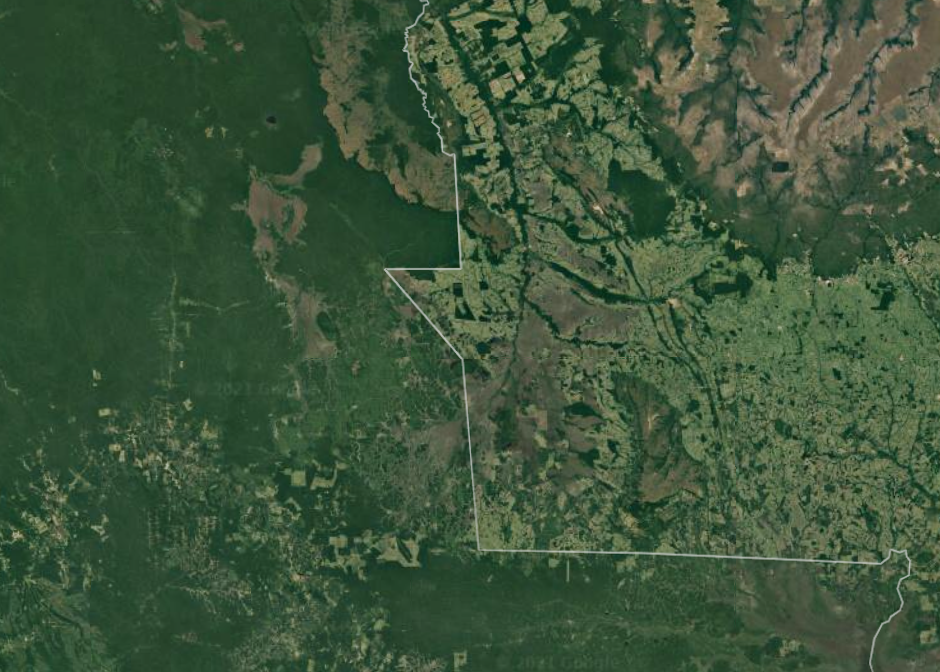
\includegraphics[width=0.8\textwidth]{../Figures/C26.2.png}
        \end{center}
        \caption{\textbf{Frontera entre Bolivia (izquierda) y Brazil}}
        \label{fig:bolivia}
    \end{figure}
\end{frame}
% ineq_ourworldindata
% 

\begin{frame}{Crecimiento y desigualdad global}
    \begin{itemize}
        \item No todas las regiones comenzaron a crecer al mismo tiempo.
        \item Durante los siglos XIX y XX, los países industrializados despegaron primero.
        \item Ex-colonias quedaron rezagadas, en parte por \textbf{instituciones extractivas} heredadas de la colonización.
        \item Esto generó una fuerte brecha entre países ricos y pobres: la “Gran Divergencia”.
        \item La desigualdad entre países aumentó de forma sostenida durante ese período.
    \end{itemize}
\end{frame}

\begin{frame}{¿Convergencia reciente?}
    \begin{itemize}
        \item En las últimas décadas, países como China, India y el sudeste asiático crecieron aceleradamente.
        \item Esto ha reducido la brecha de ingreso con los países desarrollados.
        \item La \textbf{desigualdad entre países} comenzó a disminuir en el siglo XXI.
        \item El crecimiento más rápido en economías de menor ingreso impulsa la convergencia.
        \item Resultado: \textbf{reducción masiva de la pobreza extrema} a nivel global.
    \end{itemize}
\end{frame}


\begin{frame}{Crecimiento del GDP per cápita}
    \begin{figure} [H]   
        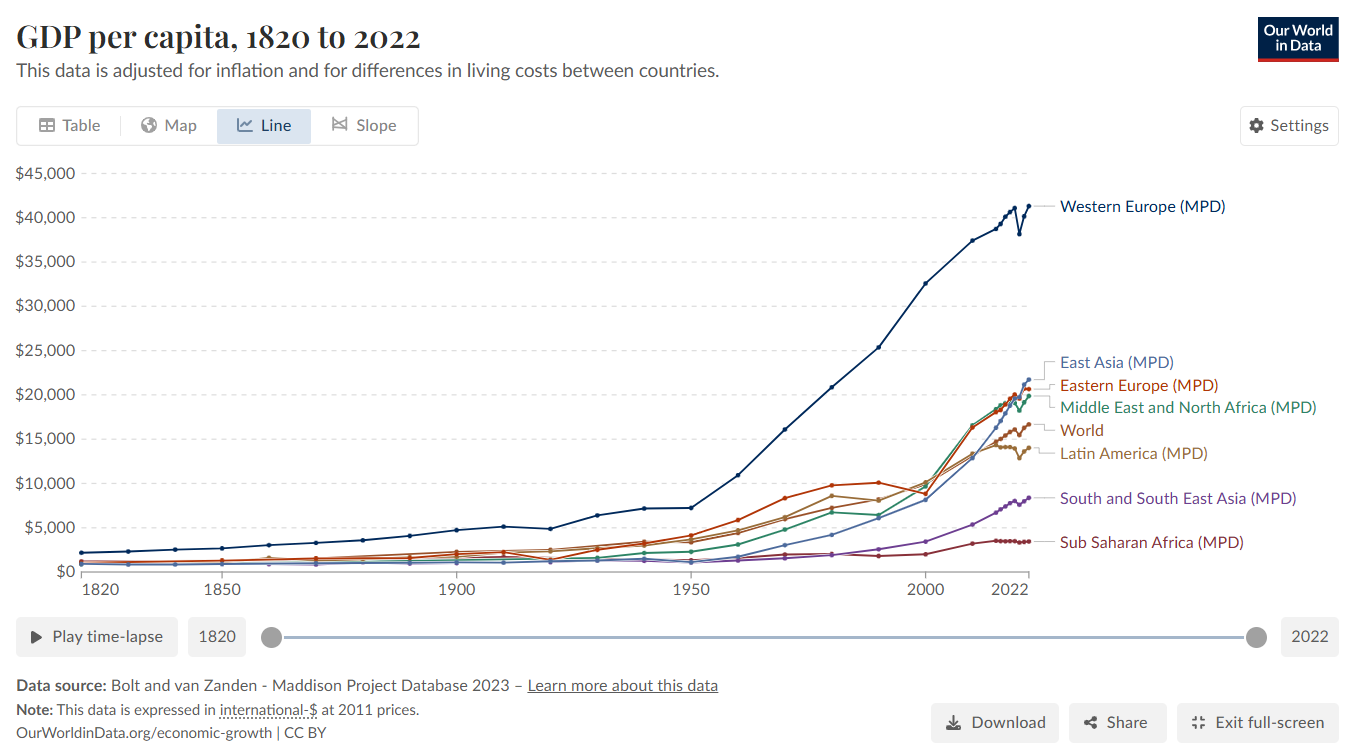
\includegraphics[scale=0.4]{../Figures/gpd_pc_ourworldindata.png}
    \end{figure}
\end{frame}

\begin{frame}{¿Qué significa “crecer”?}
    \begin{itemize}
        \item El crecimiento económico es el aumento sostenido de la producción de bienes y servicios.
        \item Se mide típicamente con el \textbf{PIB real per cápita}.
        \item ¿Pero cómo se medía el crecimiento en el pasado?
        \item Antes del siglo XX, no existía el concepto de “PIB”.
        \item Se usaban indicadores indirectos: 
        \begin{itemize}
            \item Crecimiento poblacional.
            \item Producción de alimentos básicos.
            \item Tamaño de las ciudades.
            \item Registros fiscales o eclesiásticos.
        \end{itemize}
        \item Historiadores económicos reconstruyen series usando estos datos.
    \end{itemize}
\end{frame}

\begin{frame}{Indicadores alternativos}
    \begin{itemize}
        \item Sabemos que el PIB tiene limitaciones, por ende hay alternativas que lo complementan:
        \begin{itemize}
            \item \textbf{Índice de Desarrollo Humano (IDH):} combina salud, educación e ingreso.
            \item \textbf{Índice de pobreza multidimensional.}
            \item \textbf{Indicadores de bienestar subjetivo} (“felicidad nacional bruta”).
        \end{itemize}
        \item Aún así, el PIB sigue siendo una referencia clave para comparar economías (principalmente a precios de EE.UU. - PBI PPP-).
    \end{itemize}
\end{frame}

\begin{frame}{Frontera de Posibilidades de Producción (FPP)}
    \begin{itemize}
        \item Representa las combinaciones máximas de dos bienes que puede producir una economía.
        \item Puntos sobre la curva: eficiencia productiva.
        \item Puntos dentro de la curva: desempleo o ineficiencia.
        \item Puntos fuera de la curva: inalcanzables con recursos actuales.
    \end{itemize}
\end{frame}

\begin{frame}{Gráfico: FPP simple}
    \begin{center}
        \begin{tikzpicture}[scale=1.2]
            \draw[->, very thick] (0,0) -- (6,0) node[below] {Bien A};
            \draw[->, very thick] (0,0) -- (0,6) node[left] {Bien B};
            \draw[thick, domain=0:5, smooth, variable=\x, blue] plot ({\x}, {5 - 0.2*\x*\x});
            \node at (5.3,0.3) {FPP};
            \filldraw (3,3.2) circle (2pt) node[below left] {\scriptsize Eficiente};
            \filldraw (1,1) circle (2pt) node[below] {\scriptsize Ineficiente};
            \filldraw (4.2,4) circle (2pt) node[above] {\scriptsize Inalcanzable};
        \end{tikzpicture}
    \end{center}
\end{frame}

\begin{frame}{Crecimiento económico: expansión de la FPP}
    \begin{itemize}
        \item El crecimiento económico de largo plazo se refleja en un \textbf{desplazamiento hacia afuera} de la FPP.
        \item ¿Qué lo genera?
        \begin{itemize}
            \item \textbf{Acumulación de factores productivos:} más capital (K), trabajo (L), tierra.
            \item \textbf{Tecnología y productividad:} producir más con los mismos recursos.
        \end{itemize}
        \item Ejemplo: aumento de la \textbf{inversión} en el PIB (ahorro destinado a capital) puede expandir la FPP.
        \item Ojo: no toda suba del PIB implica expansión de la FPP.
    \end{itemize}
\end{frame}

\begin{frame}{Crecimiento: expansión vs. recuperación}
    \begin{itemize}
        \item Dos formas de crecimiento del PIB:
        \begin{enumerate}
            \item \textbf{Movimiento hacia la frontera:} uso más eficiente de recursos ociosos (recuperación).
            \item \textbf{Desplazamiento de la frontera:} aumento del potencial productivo (crecimiento sostenido).
        \end{enumerate}
        \item \textbf{Pregunta frecuente:} ¿acumular capital es lo mismo que crecer?
        \begin{itemize}
            \item Si el capital se invierte en capacidad productiva: \textbf{sí, desplaza la FPP}.
            \item Si solo se acumula sin eficiencia o uso pleno: \textbf{no garantiza crecimiento sostenible}.
        \end{itemize}
        \item \textbf{Ejemplo:} recuperar empleo tras una recesión aumenta el PIB, pero no implica mayor capacidad futura.
    \end{itemize}
\end{frame}


\begin{frame}{Gráfico: desplazamiento de la FPP}
    \begin{center}
        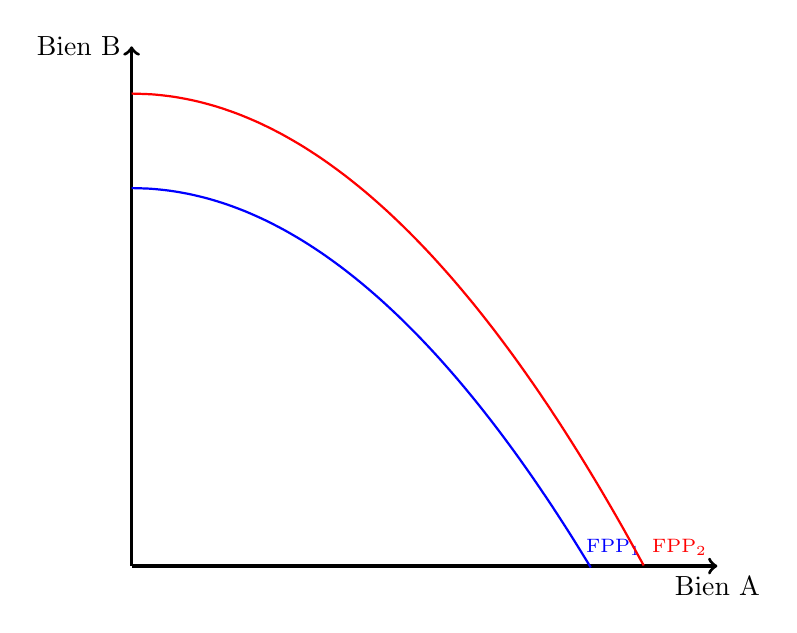
\begin{tikzpicture}[scale=1.2]
            \draw[->, very thick] (0,0) -- (6.2,0) node[below] {Bien A};
            \draw[->, very thick] (0,0) -- (0,5.5) node[left] {Bien B};
            \draw[thick, domain=0:4.86, smooth, variable=\x, blue] plot ({\x}, {4 - 0.17*\x*\x});
            \node at (5.1,0.2) {\scriptsize \textcolor{blue}{FPP$_1$}};
            \draw[thick, domain=0:5.42, smooth, variable=\x, red] plot ({\x}, {5 - 0.17*\x*\x});
            \node at (5.8,0.2) {\scriptsize \textcolor{red}{FPP$_2$}};
        \end{tikzpicture}
    \end{center}
\end{frame}

\begin{frame}{¿Qué es la productividad?}
    \begin{itemize}
        \item Es la eficiencia con la que transformamos insumos (K, L) en productos (Y).
        \item Ejemplo micro: un obrero que produce 10 sillas/día es más productivo que otro que hace 5.
        \item A nivel macro, usamos:
        \begin{itemize}
            \item Productividad laboral: PIB por trabajador.
            \item Productividad total de los factores (PTF): eficiencia conjunta de K y L.
        \end{itemize}
        \item \textbf{Pregunta:} ¿basta con más trabajo y capital para crecer sostenidamente?
    \end{itemize}
\end{frame}

\begin{frame}{Modelo de Solow: crecimiento y productividad}
    \begin{itemize}
        \item Ecuación base: $Y = A \cdot F(K, L)$
        \item $A$ representa la productividad total de los factores (PTF).
        \item En el largo plazo, $K/L$ tiende a estabilizarse \textbf{a menos que crezca $A$}.
        \item \textbf{El crecimiento sostenido requiere progreso tecnológico.}
    \end{itemize}
\end{frame}

\begin{frame}{El residuo de Solow}
    \begin{itemize}
        \item En EE.UU. posguerra: 3/4 del crecimiento no se explicaba por K ni L.
        \item Solow llamó a lo no explicado el \textbf{residuo}, es decir, la PTF.
        \item Representa: tecnología, eficiencia, organización, innovación.
        \item A veces se llama “\textit{medida de nuestra ignorancia}”.
    \end{itemize}
\end{frame}

\begin{frame}{Descomposición del crecimiento}
    \scriptsize
    \begin{itemize}
        \scriptsize
        \item Supongamos:
        \begin{itemize}
            \scriptsize
            \item PIB crece 4\% anual
            \item K y L crecen 1\% cada uno
            \item Entonces: Residuo (PTF) = 2\%
        \end{itemize}
        \item Caso Argentina 1980--2016:
        \begin{itemize}
            \scriptsize
            \item PIB per cápita creció solo 0{,}22\% anual.
            \item Capital y trabajo aportaron en promedio en forma negativa.
            \item La PTF creció algo (1{,}4\%) pero no alcanzó para impulsar el PIB.
        \end{itemize}
    \end{itemize}
    \begin{figure} [H]   
        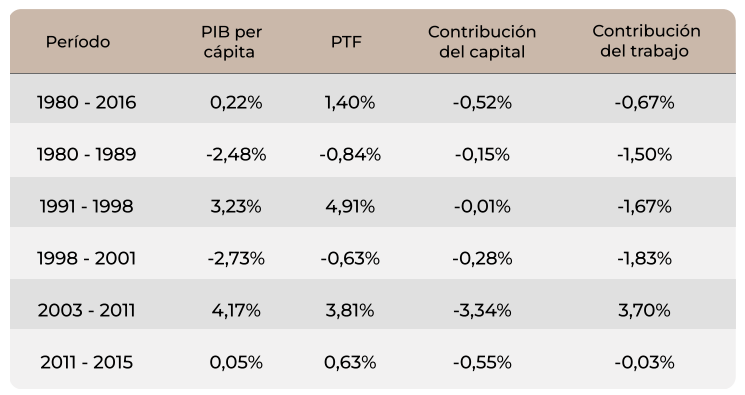
\includegraphics[scale=0.45]{../Figures/C30.8.png}
        \caption{\tiny \textbf{Descomposición del crecimiento de Argentina}}
    \end{figure}
\end{frame}

\begin{frame}{Ejemplos internacionales}
    \small
    \begin{itemize}
        \item \textbf{EE.UU.:} crecimiento impulsado principalmente por productividad y capital humano:
        \begin{itemize}
            \scriptsize
            \item Innovación tecnológica continua (I+D, patentes, Silicon Valley, sector aeroespacial).
            \item Organización empresarial moderna: mercados financieros, gerencia profesional, competencia.
            \item Educación masiva: secundaria obligatoria desde inicios del siglo XX, universidades de élite y masivas.
            \item En el análisis de Solow (1957), alrededor de 3/4 del crecimiento no se explicaba por K ni L: fue mejora de productividad (PTF).
        \end{itemize}
        \item \textbf{China:} crecimiento liderado primero por acumulación de factores, luego con mejoras de eficiencia:
        \begin{itemize}
            \scriptsize
            \item Altísima inversión en infraestructura y manufactura: ahorro interno > 40\% del PIB.
            \item Migración rural-urbana masiva: traslado de millones a sectores urbanos más productivos.
            \item Tecnología importada y aprendizaje acelerado (joint ventures, zonas económicas especiales).
            \item Entre 2011 y 2013, China vertió más cemento que EE.UU. en todo el siglo XX.
            \item En las últimas décadas, transición gradual hacia sectores intensivos en conocimiento (Huawei, BYD, AI).
        \end{itemize}
    \end{itemize}
\end{frame}


\begin{frame}{Eficiencia y equidad: conceptos clave}
    \begin{itemize}
        \item \textbf{Eficiencia:} asignación de recursos que maximiza la producción total (óptimo de Pareto).
        \item \textbf{Equidad:} justicia distributiva, cómo se reparte el ingreso entre la población.
        \item Eficiencia es el tamaño de la torta; equidad, cómo se reparte.
        \item \textbf{¿Toda redistribución reduce eficiencia?} Esta es la hipótesis del trade-off tradicional. \pause
        \item \textbf{Arthur Okun} (1975): redistribuir implica "fugas" de eficiencia.
        \item Ejemplos:
        \begin{itemize}
            \item Impuestos altos desincentivan trabajar, invertir o innovar.
            \item Transferencias pueden desalentar la oferta laboral.
            \item Costos administrativos y comportamientos oportunistas.
        \end{itemize}
        \item Metáfora del "\textbf{cubo agujereado}": parte del ingreso se pierde en el intento redistributivo.
    \end{itemize}
\end{frame}

\begin{frame}{¿Ayudar a los pobres frena el crecimiento?}
    \begin{itemize}
        \item \textit{¿Es inevitable sacrificar eficiencia para lograr más equidad?} \pause
        \item Muchos creían que sí.
        \item Pero: ¿es esta disyuntiva inevitable en el largo plazo?
        \item Nuevas evidencias ponen en duda ese trade-off. \pause
        \item FMI (Berg \& Ostry, 2011): \textbf{Menor desigualdad = crecimiento más sostenido}.
        \item ¿Por qué?
        \begin{itemize}
            \item Más gente accede a educación y oportunidades.
            \item Menos conflicto social, más estabilidad institucional.
            \item Mayor base tributaria, más inversión en bienes públicos.
        \end{itemize}
        \item \textbf{La equidad podría reforzar la eficiencia \textit{dinámica}}. No siempre es un costo.
    \end{itemize}
\end{frame}

\begin{frame}{Instrumentos para lograr eficiencia con equidad}
    \begin{itemize}
        \item Políticas que redistribuyen sin dañar productividad:
        \begin{itemize}
            \item Transferencias condicionadas (ej: Bolsa Família).
            \item Educación pública gratuita y universal.
            \item Sistemas tributarios progresivos eficientes.
        \end{itemize}
        \item \textbf{Invertir en capital humano} es equidad que también impulsa crecimiento.
    \end{itemize}
\end{frame}

\begin{frame}{Medición de la desigualdad}
    \begin{itemize}
        \item \textbf{Curva de Lorenz:} distribución acumulada del ingreso vs. población.
        \item Cuanto más se aleja de la diagonal (igualdad perfecta), más desigual es la sociedad.
        \item \textbf{Coeficiente de Gini:} 0 = igualdad perfecta, 1 = desigualdad total $\Rightarrow G=\frac{A}{A+B}$.
        \item Datos:
        \begin{itemize}
            \item Países nórdicos: Gini $\sim$ 0{,}25 (baja desigualdad).
            \item América Latina: Gini $\sim$ 0{,}50 (alta desigualdad).
        \end{itemize}
    \end{itemize}
\end{frame}

\begin{frame}{Curva de Lorenz}
    \begin{figure} [H]
    \centering
    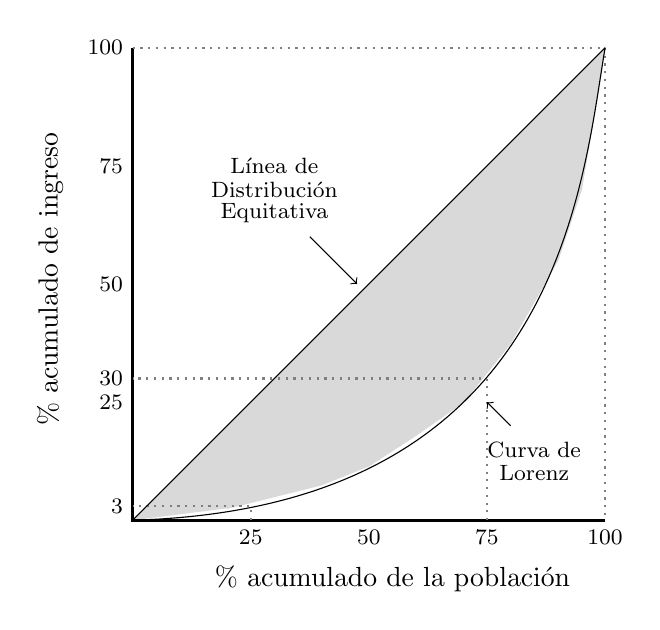
\begin{tikzpicture}[scale=0.6]
    \draw[fill,gray!30] (0,0)--(10,10)--(9.5,7)--(9,5.5)--(8,3.75)--(7,2.5)--(6,1.8)--(5,1.15)--(4,0.75)--(2,0.25);
    \draw[very thick,-] (0,10) node[above]{}--(0,0)--(10,0) node[right]{};
    \draw[thick, dotted, gray] (0,10)--(10,10)--(10,0);
    \draw[thick, dotted, gray] (2.5,0)--(2.5,0.3)--(0,0.3);
    \draw[thick, dotted, gray] (7.5,0)--(7.5,3)--(0,3);
    \draw[thin] (0,0)--(10,10);
    \draw[thin] (0,0)..controls (9,0.25) and (9.5,7)..(10,10);
    \node at (-1.75, 5){\rotatebox{90}{ \% acumulado de ingreso}};
    \node[] at (5.5,-1.25) { \% acumulado de la población};
    \node[below] at (2.5,0){\footnotesize 25};
    \node[below] at (5,0){\footnotesize 50};
    \node[below] at (7.5,0){\footnotesize 75};
    \node[below] at (10,0){\footnotesize 100};
    \node[left] at (0,0.3){\footnotesize 3};
    \node[left] at (0,2.5){\footnotesize 25};
    \node[left] at (0,3){\footnotesize 30};
    \node[left] at (0,5){\footnotesize 50};
    \node[left] at (0,7.5){\footnotesize 75};
    \node[left] at (0,10){\footnotesize 100};
    \node[] at (3,7.5) {\footnotesize Línea de };
    \node[] at (3,7) {\footnotesize Distribución};
    \node[] at (3,6.5) {\footnotesize Equitativa };
    \draw[thin, ->] (3.75,6)--(4.75,5);
    \node[] at (8.5,1.5) {\footnotesize Curva de };
    \node[] at (8.5,1) {\footnotesize Lorenz };
    \draw[thin, ->] (8,2)--(7.5,2.5);
    \end{tikzpicture}
    \end{figure}
\end{frame}

\begin{frame}{Reflexión final: ¿crecer primero y repartir después?}
    \begin{itemize}
        \item La evidencia sugiere que \textbf{distribuir bien desde el principio puede ayudar a crecer}.
        \item La desigualdad excesiva erosiona el contrato social, genera inestabilidad y desconfianza.
        \item \textbf{Crecimiento inclusivo:} que sus beneficios lleguen a amplios sectores.
        \item Instituciones inclusivas promueven \textbf{equidad y crecimiento} de forma sostenible.
    \end{itemize}
\end{frame}







\begin{comment}
\begin{frame}
\frametitle{Tomemos una economía}
\begin{center}
    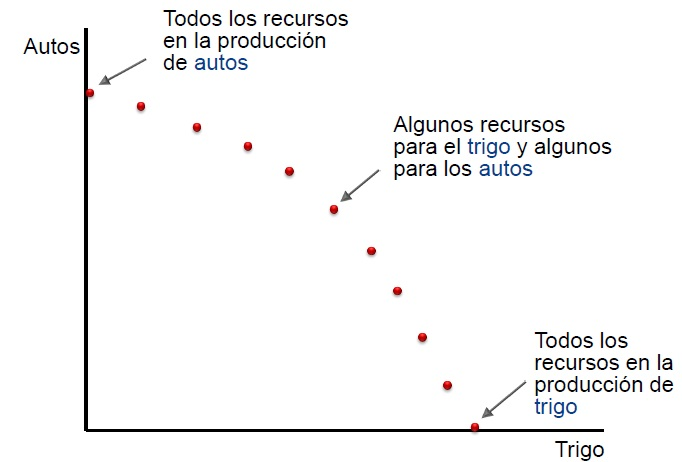
\includegraphics[scale=0.6]{../Figures/Tema_11.2_tomemosunaeconomia.jpg}
\end{center}
\end{frame}

\begin{frame}
\frametitle{Frontera de posibilidades}
\begin{center}
    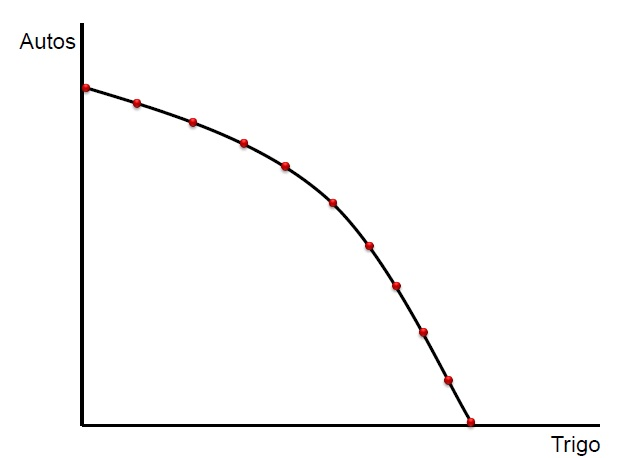
\includegraphics[scale=0.6]{../Figures/Tema_11.3_frontera.jpg}
\end{center}
\end{frame}

\begin{frame}
\frametitle{Frontera de posibilidades}
\begin{center}
    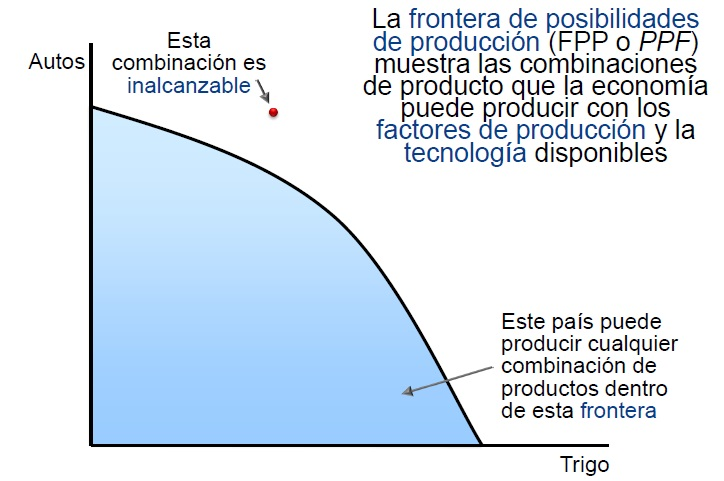
\includegraphics[scale=0.55]{../Figures/Tema_11.4_fronteradeposibilidades.jpg}
\end{center}
\end{frame}

\begin{frame}
\frametitle{Fuera de la frontera}
\begin{center}
    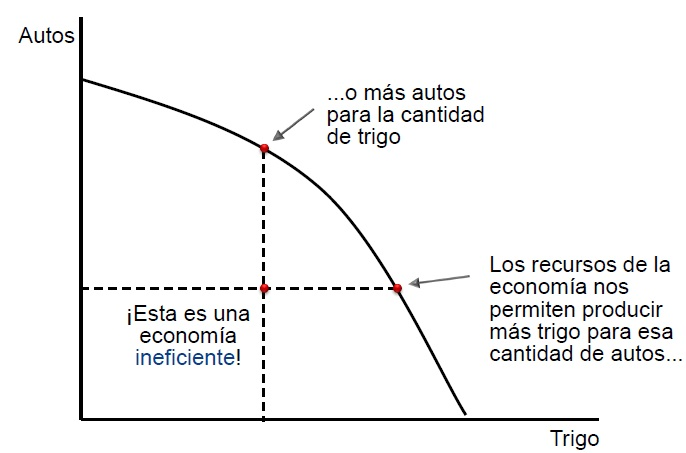
\includegraphics[scale=0.6]{../Figures/Tema_11.5_fueradelafrontera.jpg}
\end{center}
\end{frame}

\begin{frame}
\frametitle{Misma frontera}
\begin{center}
    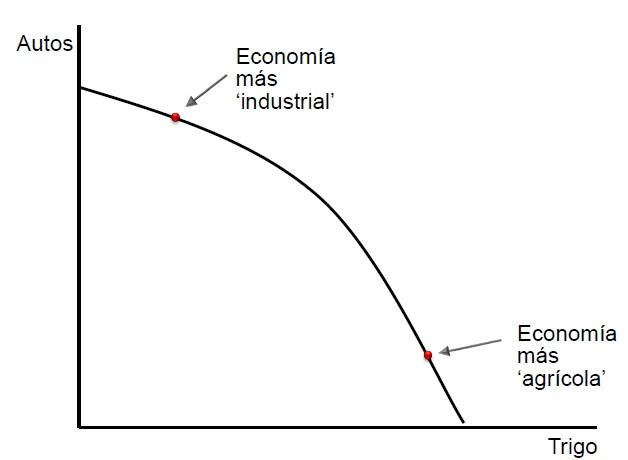
\includegraphics[scale=0.6]{../Figures/Tema_11.6_lamismafrontera.jpg}
\end{center}
\end{frame}

\begin{frame}
\frametitle{Cambio en la tecnología}
\begin{center}
    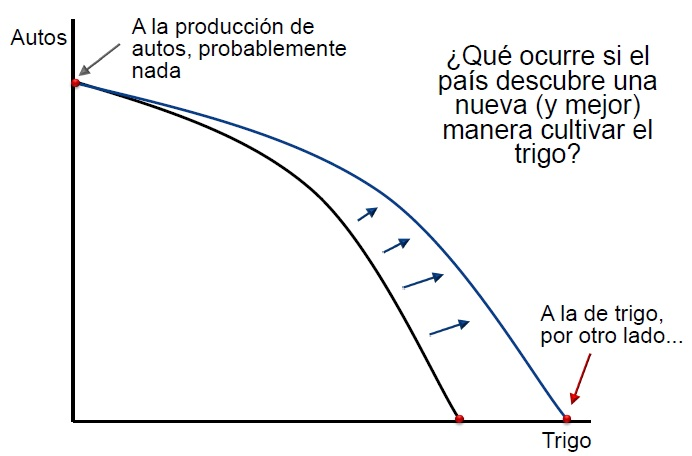
\includegraphics[scale=0.6]{../Figures/Tema_11.7_cambiotecnologico.jpg}
\end{center}
\end{frame}

\begin{frame}
\frametitle{Cambio en los factores}
\begin{center}
    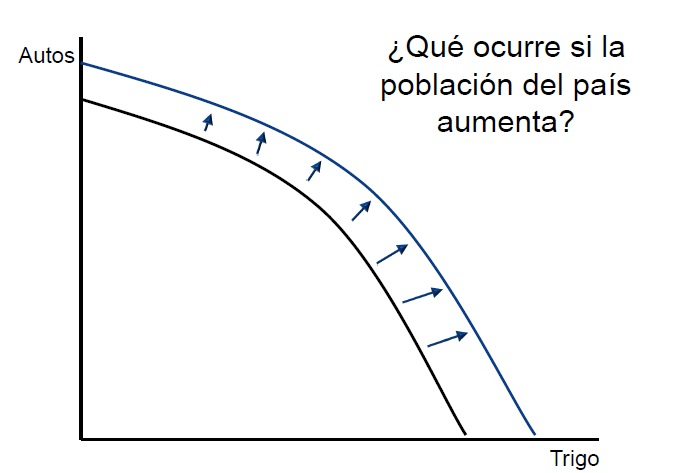
\includegraphics[scale=0.55]{../Figures/Tema_11.8_cambioenlosfactores.jpg}
\end{center}
\end{frame}

\begin{frame}
\frametitle{Shock exógeno}
\begin{center}
    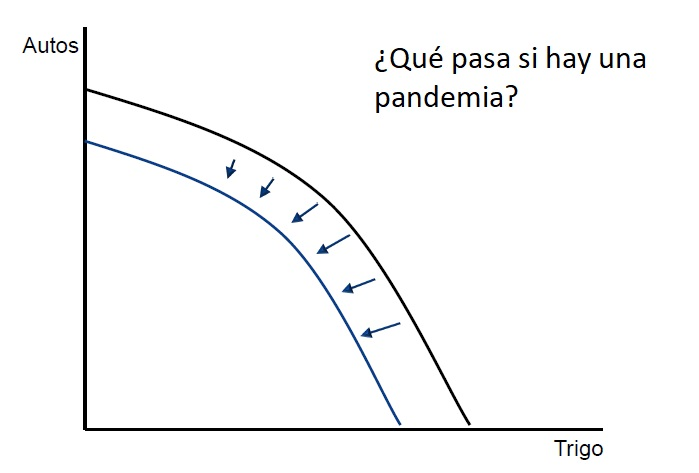
\includegraphics[scale=0.6]{../Figures/Tema_11.9_pandemia.jpg}
\end{center}
\end{frame}

\begin{frame}
\frametitle{Cambios en el equilibrio}
\begin{center}
    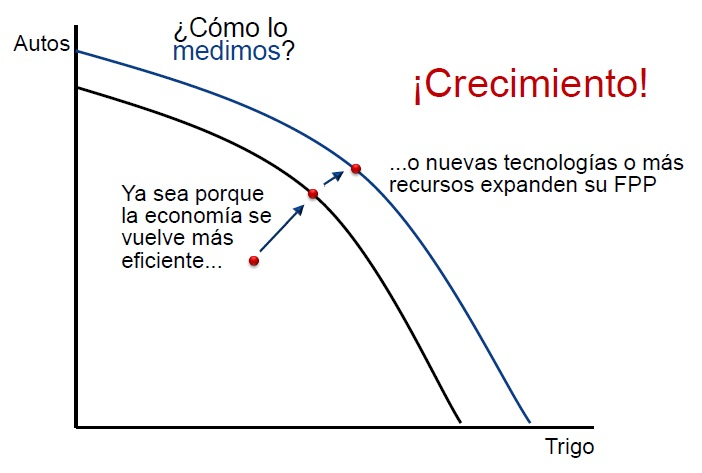
\includegraphics[scale=0.6]{../Figures/Tema_11.10_crecimiento.jpg}
\end{center}
\end{frame}

\begin{frame}
\frametitle{Luces nocturnas}
\begin{center}
    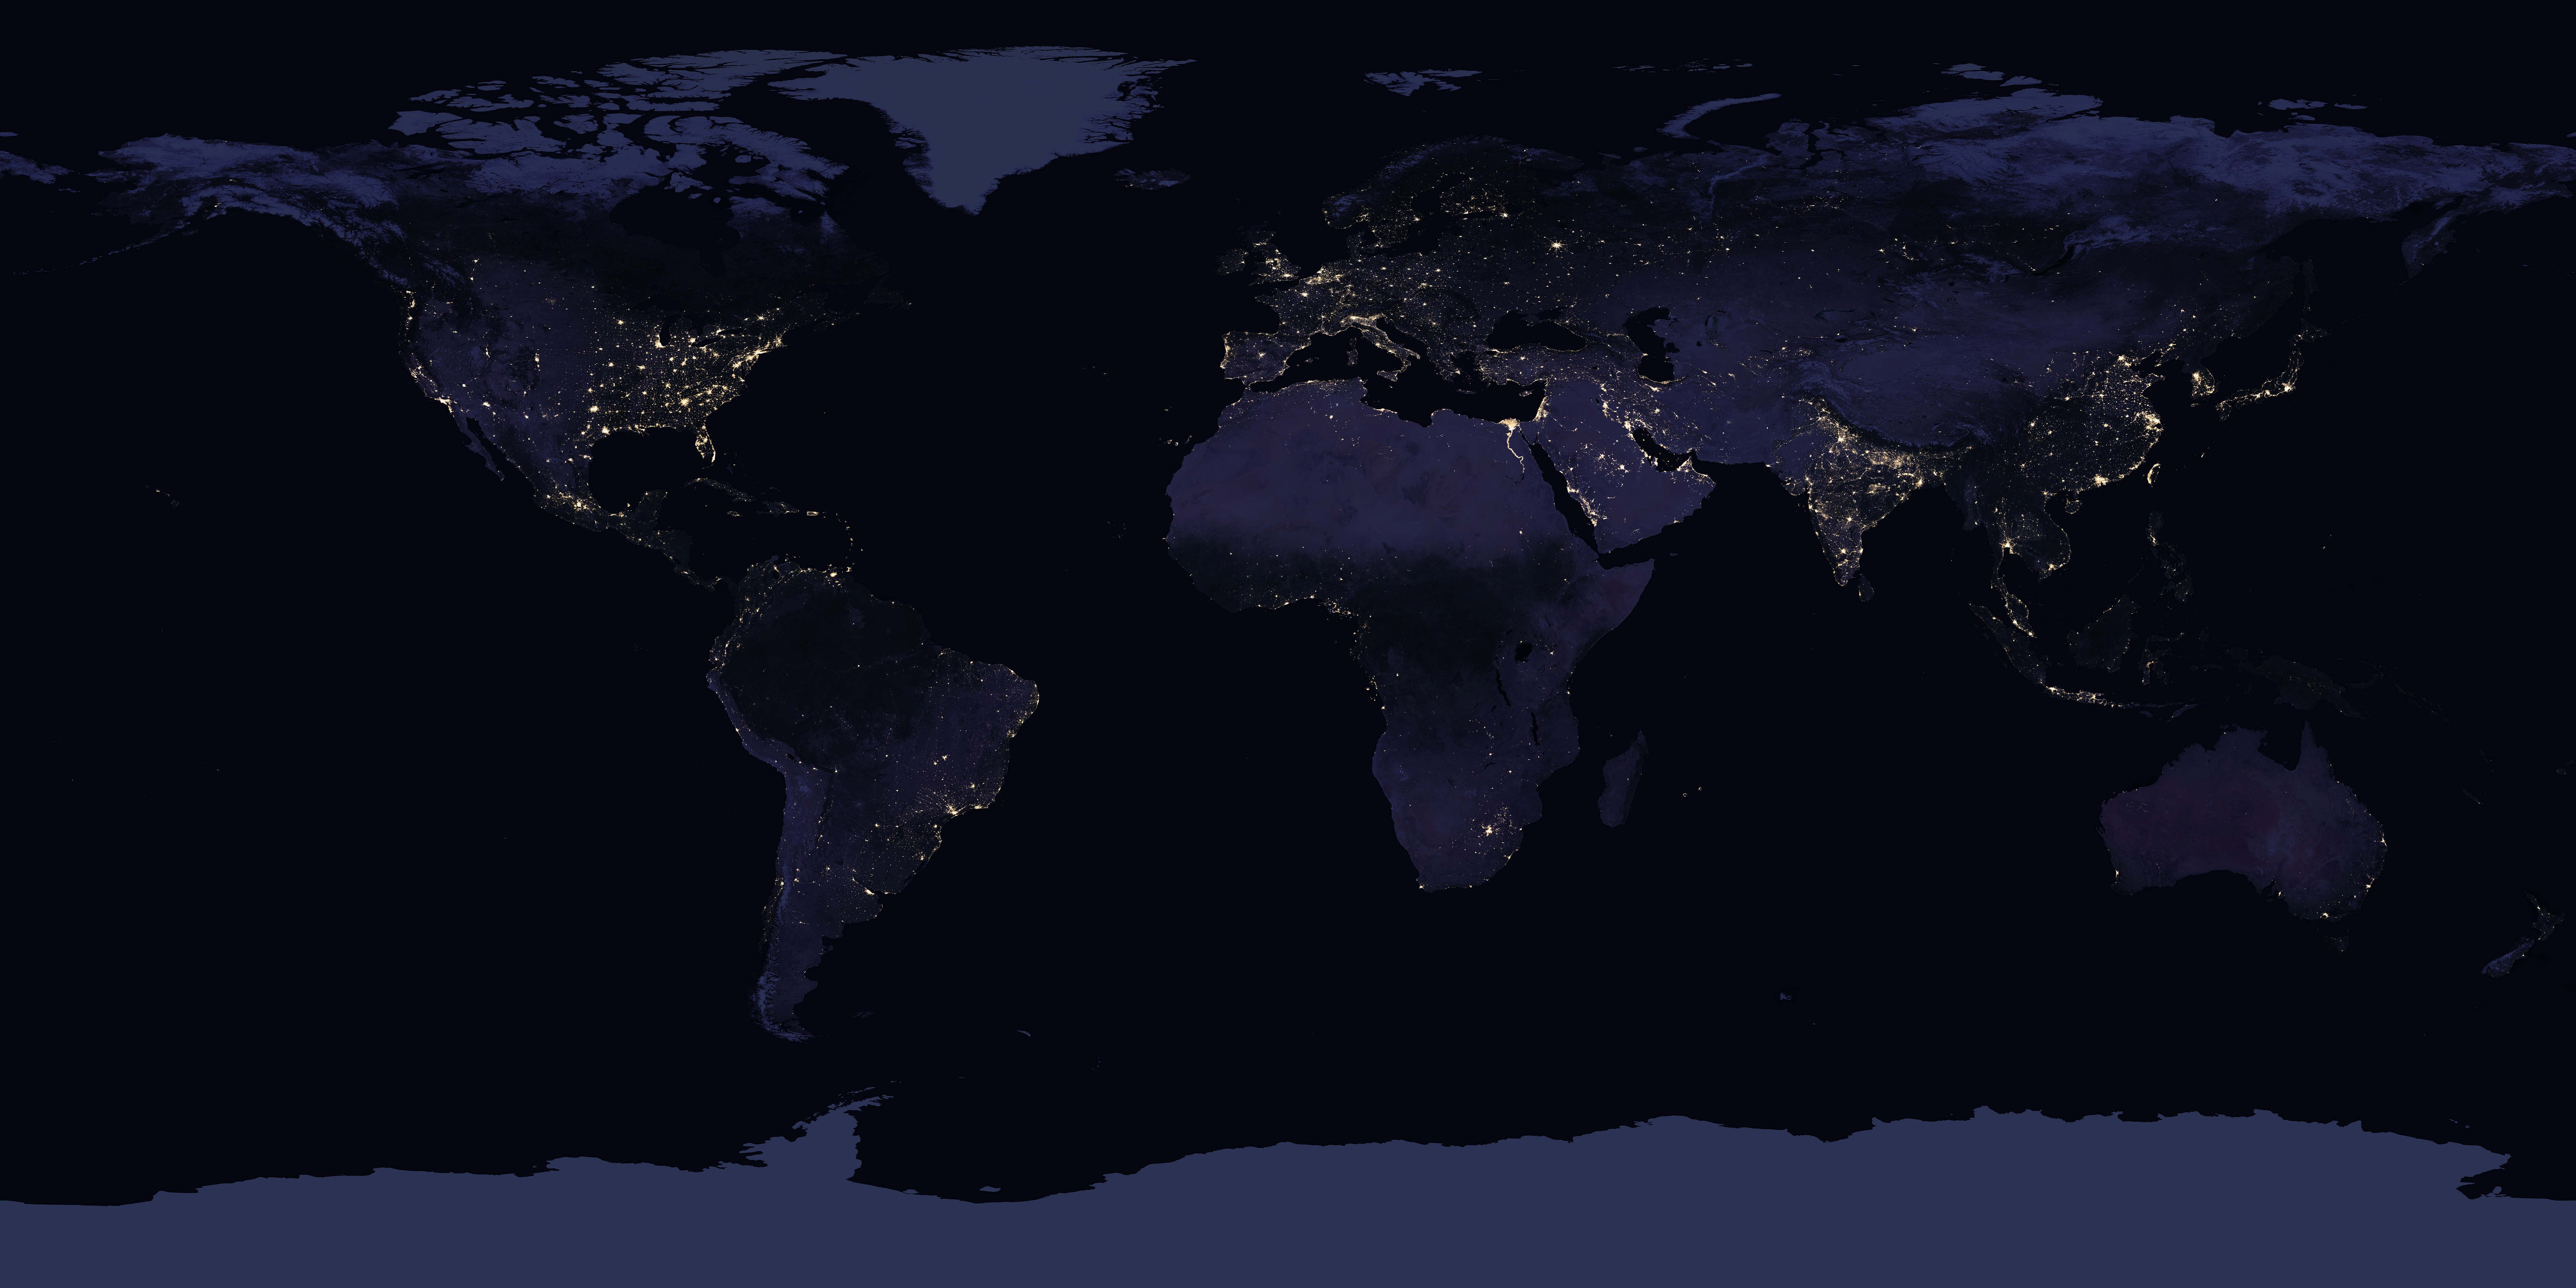
\includegraphics[scale=0.06]{../Figures/Tema_11.11_crecimiento2.jpg}
\end{center}
Fuente: \href{https://www.nasa.gov/feature/goddard/2017/new-night-lights-maps-open-up-possible-real-time-applications}{NASA}
\end{frame}

\begin{frame}
\frametitle{Crecimiento}
\begin{center}
    \href{https://ourworldindata.org/grapher/gdp-per-capita-worldbank} {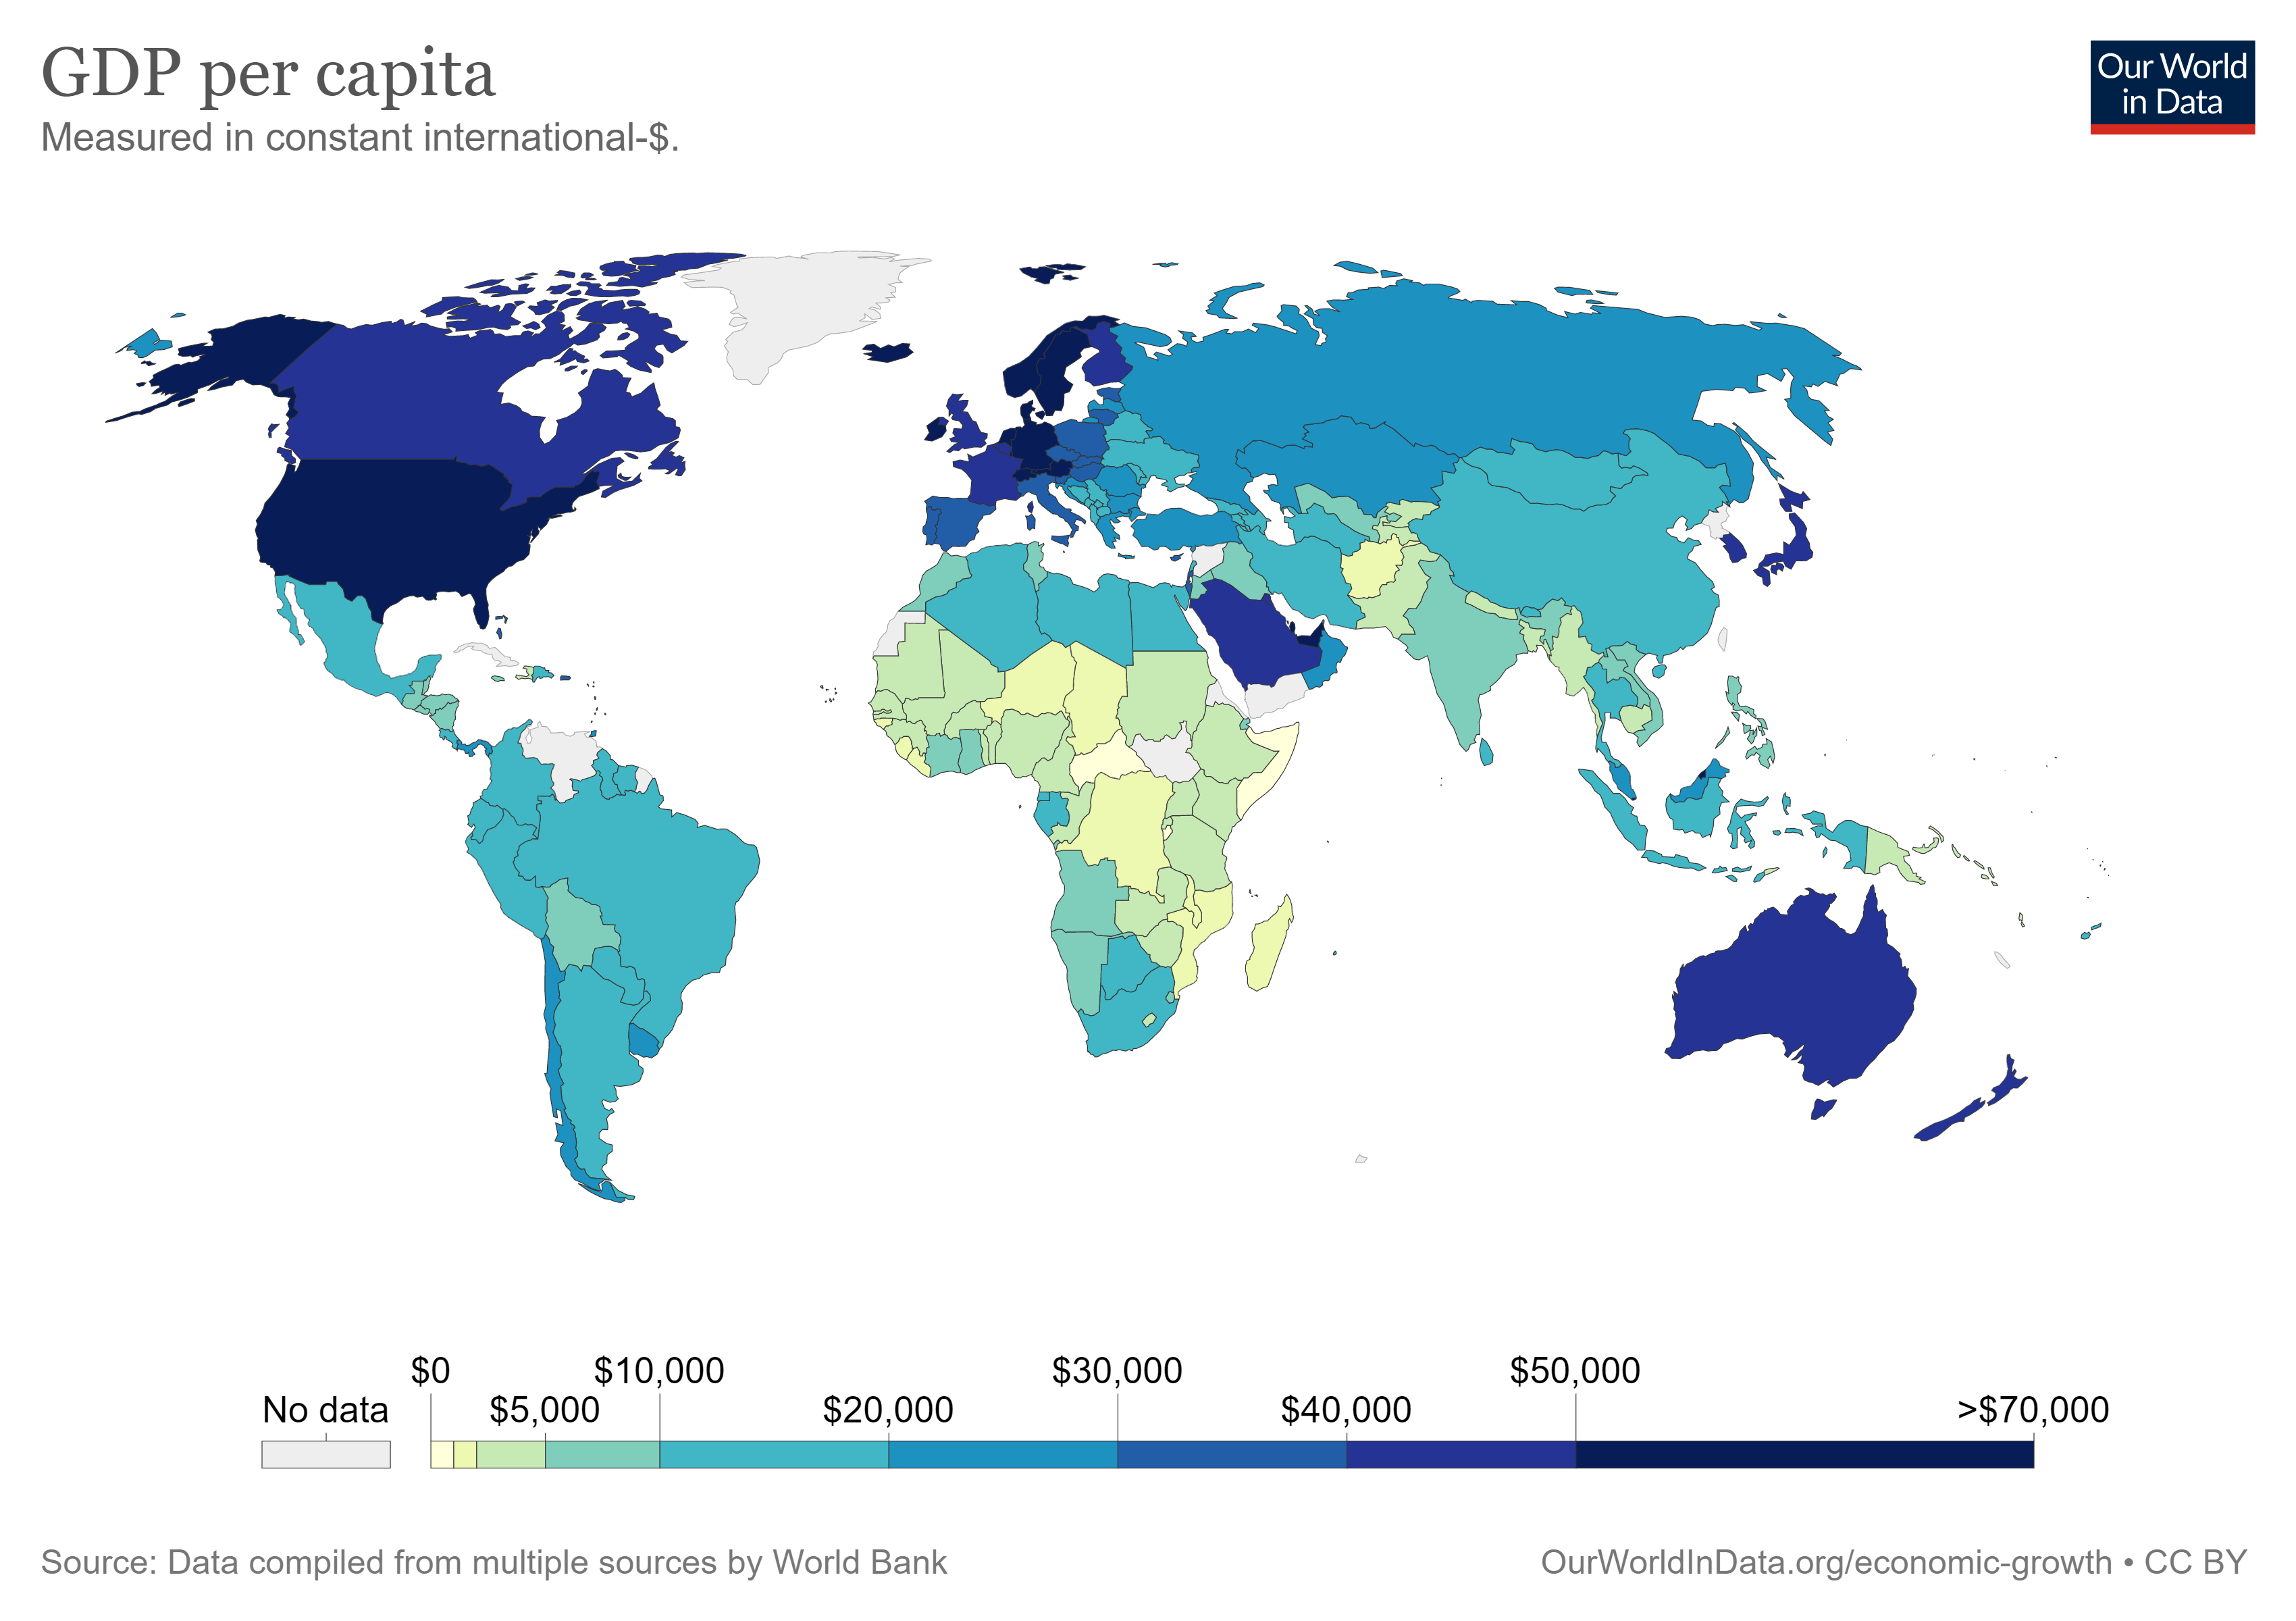
\includegraphics[width=0.8\textwidth]{../Figures/gdppc2020.png}}
\end{center}
Fuente: Our World in Data
\end{frame}

\begin{frame}{¿Qué generó el crecimiento explosivo?}
    \begin{itemize}
    \item \textbf{Revolución industrial (desde mediados del Siglo XVIII)}
    \begin{itemize}
        \item La máquina a vapor generó una potencialidad de expansión en la producción junto con los ferrocarriles y la industria textil produjeron un aumento en el nivel de vida sin precedentes
    \end{itemize}
    \item \textbf{Constitución de EEUU (1787)}
     \begin{itemize}
        \item Fuerte contraste con el poder absolutista de los monarcas europeos
        \item Fuertes restricciones al Estado y lo que éste podía hacer
        \item La emergencia de los gobiernos republicanos con división de poderes implicó un cambio radical en la calidad de la gestión de los recursos públicos
    \end{itemize}
    \item \textbf{Revolución francesa (1789)}
    \begin{itemize}
        \item Permitió la movilidad social
        \item Se pasó de una sociedad estamental a una sociedad libre: mayor libertad para elegir los trabajos y ocupaciones según sus preferencias y capacidades
    \end{itemize}
\end{itemize}
\end{frame}

%\begin{frame}{Felicidad y nivel de ingreso}
%    \begin{figure} [H]   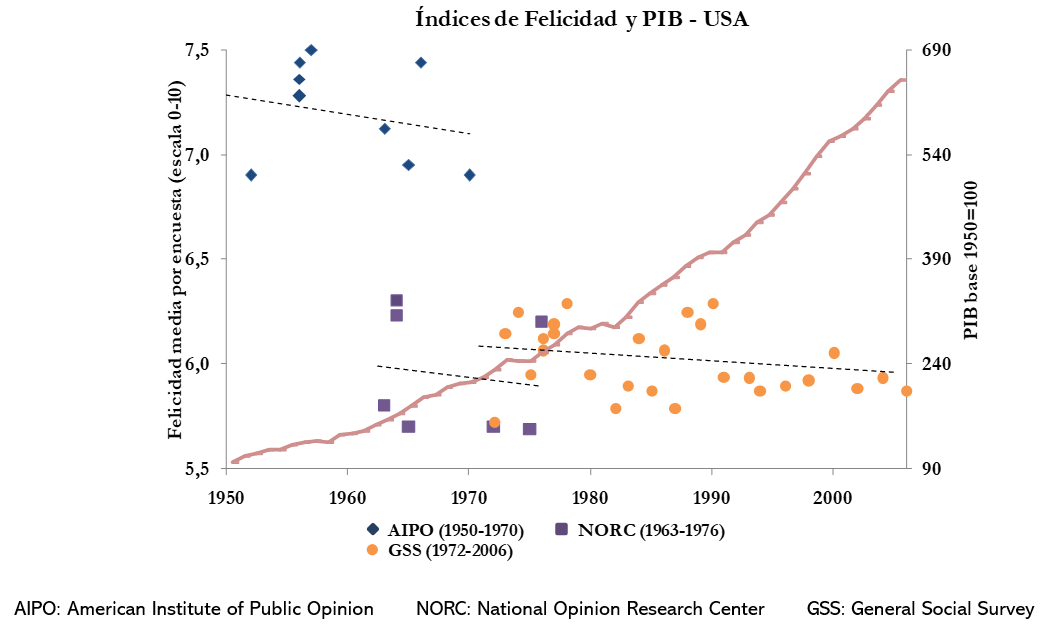
\includegraphics[scale=0.5]{../Figures/C17.2.png}
%\end{figure}
%\end{frame}

%\begin{frame}
%\frametitle{Idea más amplia de bienestar}
%\begin{itemize}
%    \item Enfoque de capacidades de Amartya Sen
%    \begin{itemize}
%        \item No es lo que una persona tiene, sino lo que ella es y puede hacer \\
%        - Capacidades para alcanzar su potencial como ser humano
%        \item ¿Disparidad entre los ingresos y las ventajas reales? \\
%        - Heterogeneidades personales, diversidad ambiental, diferencias en el clima social, distribución de recursos dentro de la familia, etc.
%    \end{itemize}
%    \item Índice de Desarrollo Humano (HDI) del PNUD
%    \begin{itemize}
%        \item Ingresos (PBI per cápita ajustado por PPP)
%        \item Longevidad (esperanza de vida al nacer)
%        \item Conocimiento (alfabetización y años de estudio0
%    \end{itemize}
%    \end{itemize}
%\end{frame}

%\begin{frame}
%\frametitle{HDI (2017)}
%\begin{center}
%    \href{https://ourworldindata.org/grapher/human-development-index?country=~ZWE} {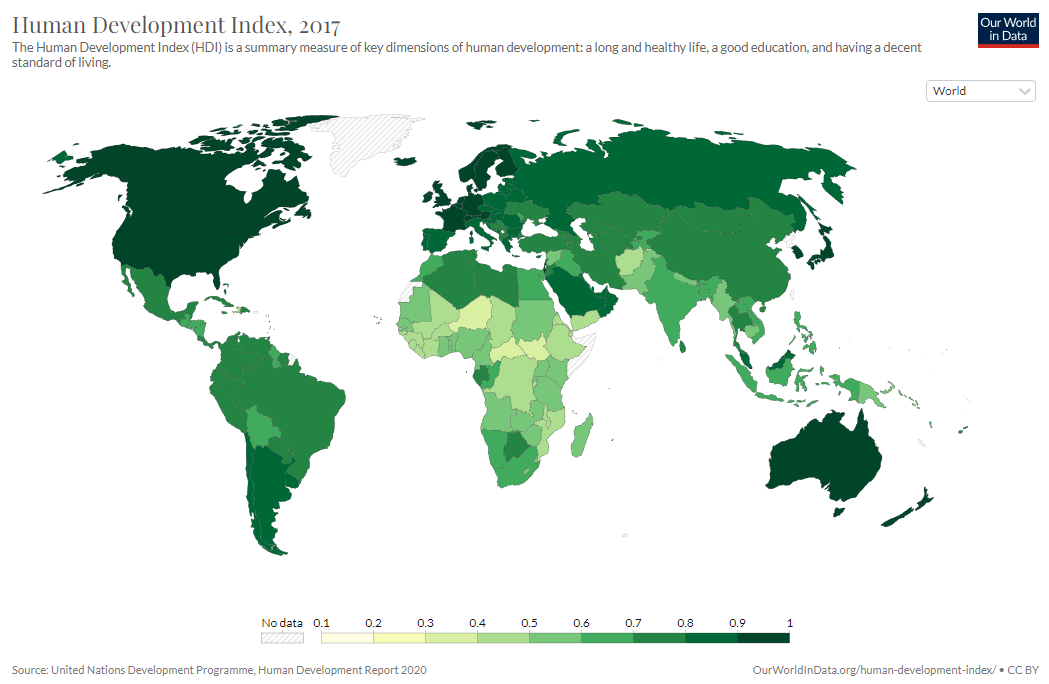
\includegraphics[scale=0.35]{../Figures/Tema_11.27_hdi_PBI.png}}
%\end{center}
%Fuente: Our World in Data
%\end{frame}

\begin{frame}
\frametitle{PBI y desarrollo}
\begin{center}
    \href{https://ourworldindata.org/grapher/hdi-vs-gdp-per-capita} {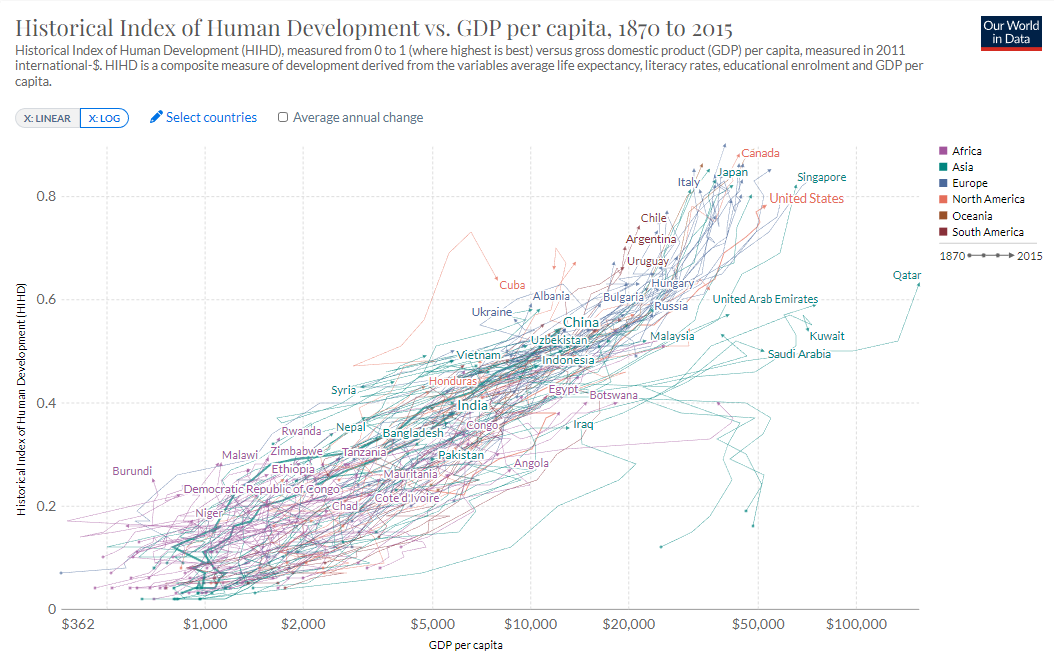
\includegraphics[scale=0.35]{../Figures/Tema_11.27_hdi_2.png}}
\end{center}
Fuente: Our World in Data
\end{frame}

\begin{frame}{Fuentes del crecimiento}
   \begin{equation}
    Y = A\,F(K,L,H,RN)
\end{equation} 
\begin{itemize}
    \item El crecimiento viene de la acumulacion de factores o de la tecnologia?
    \item El hallazgo de Solow: la acumulacion de factores no es suficiente para explicar el crecimiento.
\end{itemize}
\end{frame}

\begin{frame}{Un ejemplo de productividad}
    \begin{figure} [H]   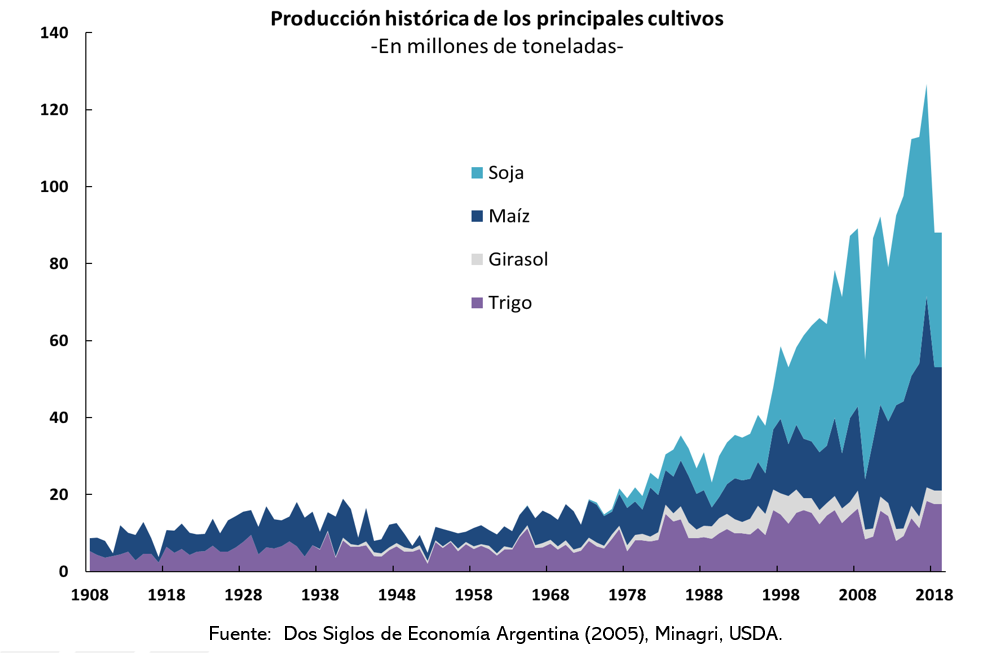
\includegraphics[scale=0.55]{../Figures/C17.3.png}
\label{fig:17.3}
\end{figure}
\end{frame}


\begin{frame}{La descomposición de crecimiento para Argentina}
    \begin{figure} [H]   
        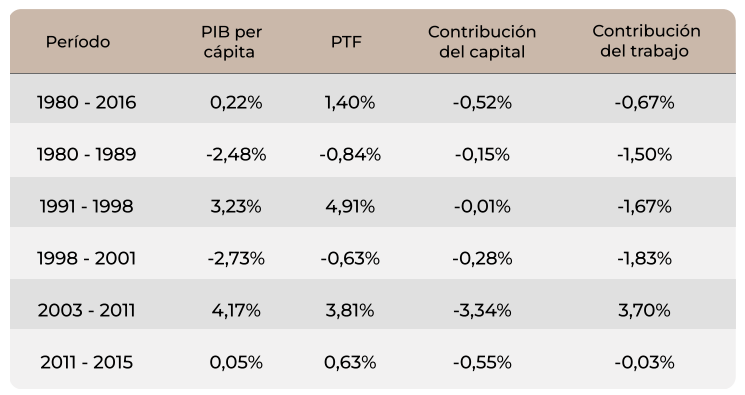
\includegraphics[scale=0.55]{../Figures/C30.8.png}
        \caption{\textbf{Descomposición del crecimiento de Argentina}}
    \end{figure}
\end{frame}

\begin{frame}{Instituciones y Crecimiento}
    \begin{itemize}
        \item Dijimos que las instituciones son las reglas del juego en una sociedad
        \item \textbf{Instituciones económicas e instituciones políticas}
        \item Afectan de manera directa a los incentivos
        \item Establecen los incentivos para la innovación y el desarrollo tecnológico
        \item ¿Podemos evaluar de manera empírica el rol de las instituciones?
    \end{itemize}
    
    \begin{figure}[H]
        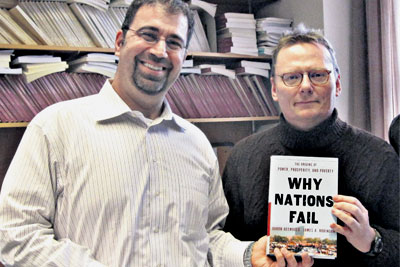
\includegraphics[scale=0.5]{../Figures/Acemoglurobinson.png}
    \end{figure}
\end{frame}


\begin{frame}{Desigualdad del Ingreso}
        \begin{itemize}
            \item Hay dos criterios para evaluar una asignación específica: 
            \begin{itemize}
                \item Eficiencia
                \item Equidad
            \end{itemize}
            \item ¿Existe un trade off entre eficiencia y equidad?
            \item Hay algunos factores importantes que determinan si una asignación es muy desigual:
            \begin{itemize}
                \item Diferencias en el poder de negociación
                \item Diferencias en sus dotaciones
                \item Instituciones
            \end{itemize}
            \item Para evaluar la desigualdad, los economistas a menudo usan unas medidas llamadas Coeficiente de Gini y Curva de Lorenz.
        \end{itemize}
\end{frame}

\begin{frame} 
\frametitle{La curva de Lorenz}
\begin{itemize}
\item Es una herramienta útil para observar la distribución completa del ingreso o la riqueza que representa y comparar las distribuciones del ingreso o la riqueza entre los países
\item Es una representación gráfica de la desigualdad de cierta cantidad, como la riqueza o el ingreso
\item Indica cuánta disparidad hay en el ingreso, o en cualquier otra medida, a través de la población
\end{itemize}
\end{frame}

\begin{frame} 
\frametitle{La curva de Lorenz}
\begin{itemize}
\item Los individuos se organizan en orden ascendente según el ingreso que tienen, y la parte acumulada del ingreso se grafica contra la parte acumulada de la población
\item Para la igualdad completa de ingresos, la curva de Lorenz sería una línea recta con una pendiente igual a uno
\item La medida en que la curva cae por debajo de esta línea de igualdad perfecta es una medida de la desigualdad
\end{itemize}
\end{frame}

\begin{frame} 
\frametitle{Curva de Lorenz}
\begin{figure} [H]
\centering
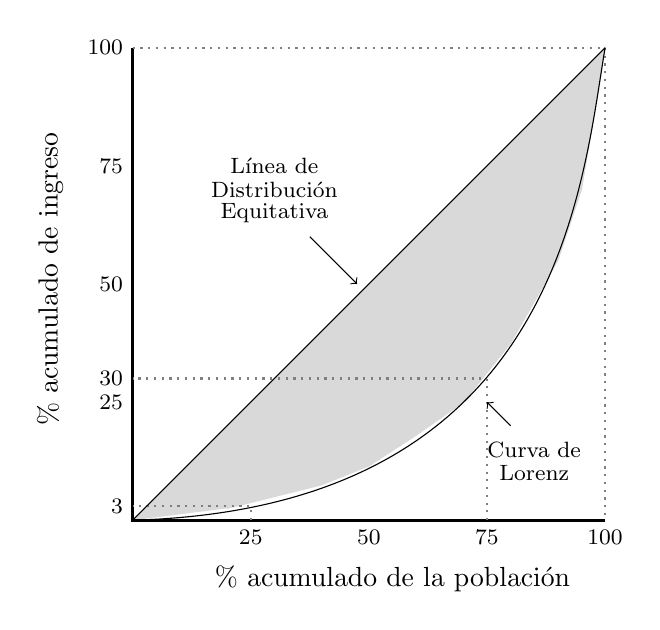
\begin{tikzpicture}[scale=0.6]
\draw[fill,gray!30] (0,0)--(10,10)--(9.5,7)--(9,5.5)--(8,3.75)--(7,2.5)--(6,1.8)--(5,1.15)--(4,0.75)--(2,0.25);
\draw[very thick,-] (0,10) node[above]{}--(0,0)--(10,0) node[right]{};
\draw[thick, dotted, gray] (0,10)--(10,10)--(10,0);
\draw[thick, dotted, gray] (2.5,0)--(2.5,0.3)--(0,0.3);
\draw[thick, dotted, gray] (7.5,0)--(7.5,3)--(0,3);
\draw[thin] (0,0)--(10,10);
\draw[thin] (0,0)..controls (9,0.25) and (9.5,7)..(10,10);
\node at (-1.75, 5){\rotatebox{90}{ \% acumulado de ingreso}};
\node[] at (5.5,-1.25) { \% acumulado de la población};
\node[below] at (2.5,0){\footnotesize 25};
\node[below] at (5,0){\footnotesize 50};
\node[below] at (7.5,0){\footnotesize 75};
\node[below] at (10,0){\footnotesize 100};
\node[left] at (0,0.3){\footnotesize 3};
\node[left] at (0,2.5){\footnotesize 25};
\node[left] at (0,3){\footnotesize 30};
\node[left] at (0,5){\footnotesize 50};
\node[left] at (0,7.5){\footnotesize 75};
\node[left] at (0,10){\footnotesize 100};
\node[] at (3,7.5) {\footnotesize Línea de };
\node[] at (3,7) {\footnotesize Distribución};
\node[] at (3,6.5) {\footnotesize Equitativa };
\draw[thin, ->] (3.75,6)--(4.75,5);
\node[] at (8.5,1.5) {\footnotesize Curva de };
\node[] at (8.5,1) {\footnotesize Lorenz };
\draw[thin, ->] (8,2)--(7.5,2.5);
\end{tikzpicture}
\end{figure} 
\end{frame}

\begin{frame} 
\frametitle{El coeficiente de Gini y la curva de Lorenz}
\begin{itemize}
\item Si todos tienen el mismo ingreso (no hay desigualdad de ingresos), el coeficiente de Gini toma un valor de 0.
\item Esto se debe a que la curva de Lorenz sería exactamente la línea de la igualdad perfecta, por lo que no habría área entre los dos
\item $G=\frac{A}{A+B}$
\item Este método de cálculo del Gini solo da una aproximación. La aproximación del área sólo es precisa cuando la población es grande
\end{itemize}
\end{frame}

\begin{frame} 
\frametitle{Un ejemplo aplicado}
    \begin{center}    
    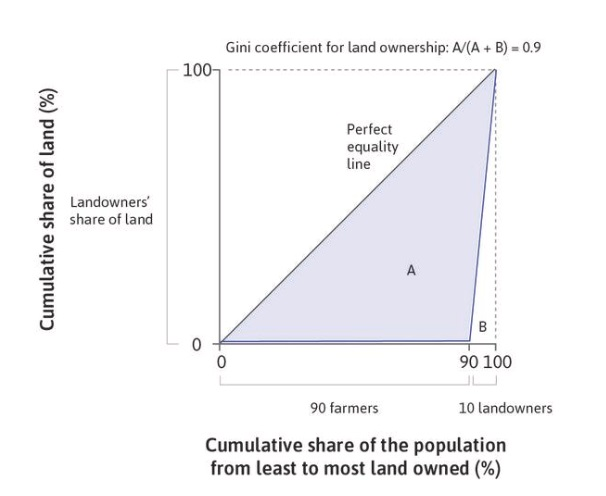
\includegraphics[scale=0.55]{../Figures/Tema_04.18_lorenz3.jpg}
    \end{center}
\end{frame}

\begin{frame} 
\frametitle{Un ejemplo aplicado}
    \begin{center}    
    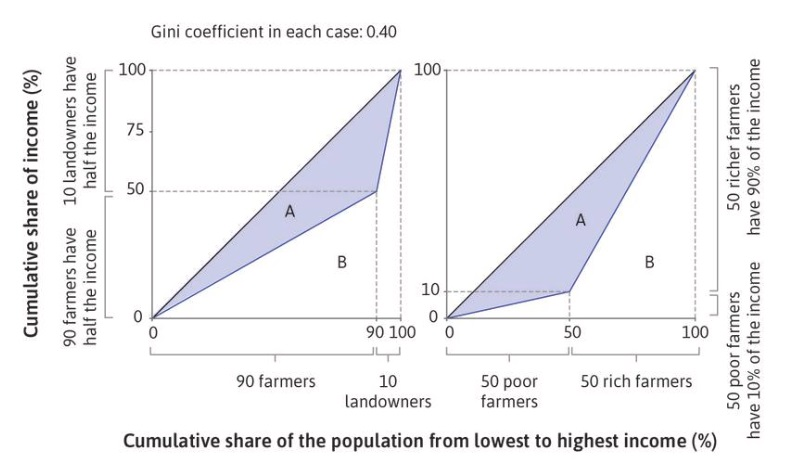
\includegraphics[scale=0.55]{../Figures/Tema_04.20_variedaddesigual.jpg}
    \end{center}
\end{frame}

\begin{frame} 
\frametitle{Diferentes variedad de desigualdad}
\begin{itemize}
\item En la figura anterior hay dos sociedades con el mismo coeficiente de Gini.
\item El área $\frac{A}{A + B}$ es la misma en cada curva de Lorenz, pero la distribución del ingreso está lejos de ser idéntica.
\item En la sociedad de la izquierda, la mitad del ingreso total se divide entre 90 agricultores mientras que 10 terratenientes obtienen la mitad restante. 
\item En la sociedad que se muestra a la derecha, 50 agricultores pobres obtienen una décima parte de los ingresos para dividirse entre ellos y 50 agricultores más ricos dividen el 90\% restante.
\end{itemize}
\end{frame}

\begin{frame} 
\frametitle{Diferentes variedad de desigualdad}
\begin{itemize}
\item ¡No todas las desigualdades son iguales!
\item No es lo mismo que una sociedad sea altamente desigual porque hay un pequeño número de personas excepcionalmente ricas y todos los demás están en una situación de buena posición económica o que sea desigual porque hay un pequeño número de personas muy pobres, y todos los demás están en mejores condiciones
\item Estas dos sociedades podrían tener el mismo coeficiente de Gini, pero pensaríamos que son bastante diferentes en la naturaleza de la desigualdad que experimentan
\end{itemize}
\end{frame}
\end{comment}
\end{document}